\chapter{Teaching Your PI Controller to Behave (Part IV)}

At the end of my last blog, we discussed the possibility of creating a single parameter that could automatically tune the PI coefficients for a velocity loop used in a motor speed control system.  To develop such a parameter, let’s review the open-loop transfer function for the entire velocity loop:

\begin{equation}\label{eq:4_1}
    GH(s) = \frac{KK_cK_d\left(1+\frac{s}{K_d}\right)}{s^2\left(1+\frac{L}{K_a}s\right)\left(1+\tau s\right)}
\end{equation}
where
\begin{itemize}
    \item $K$ is a coefficient that contains several terms related to the motor and load
    \item $K_c$ and $K_d$ are the PI coefficients for the velocity loop
    \item $L$ is the motor inductance
    \item $K_a$ is one of the PI coefficients for the current loop
    \item $\tau$ is the time constant of the velocity feedback filter
    \item $s$ is the Laplace frequency variable
\end{itemize}

Assuming that the zero \unit{\dB} frequency occurs somewhere between the zero at $s = K_d$ and the two nonzero poles in the denominator of the expression, we should end up with a Bode plot that looks something like this:


\begin{center}
    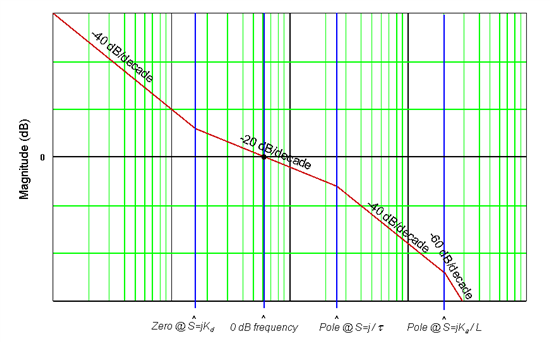
\includegraphics[width=1\linewidth]{04/01_bode}
\end{center}

The reason the shape of this curve is so important is because the phase shift at the \qty{0}{\dB} frequency determines the stability of the system.  In general, in order to get a phase shift at \qty{0}{\dB} that leads to good stability, the magnitude response should cross \qty{0}{\dB} at a rate no steeper than \qty{-20}{\dB\per\decade}.

As you can see from \ref{eq:4_1}, we must solve for three unknowns ($K_a$, $K_c$, and $K_d$) which are affected by multiple system parameters.  But instead of wading through pages and pages of esoteric equations, it’s time to make another simplification.  Let’s assume that there is only \textit{one} pole higher than the zero-dB frequency instead of two.  This assumption could mean that you don’t have a velocity filter in your system, OR that the velocity filter’s pole is \textit{way} higher than the current controller’s pole, OR that the current controller’s pole is \textit{way} higher than the velocity filter’s pole.  For most systems, it is plausible to assume the latter scenario.  So if we eliminate the effect of the current controller pole, we can rewrite the velocity open-loop transfer function as shown below:

\begin{equation}\label{eq:4_2}
    GH(s) = \frac{KK_cK_d\left(1+\frac{s}{K_d}\right)}{s^2 \left(1+\tau s\right)}
\end{equation}

For now, let’s assume that the delta in frequency between the pole $1/\tau$ and the zero $K_d$ is fixed.  In order to achieve maximum phase margin (phase shift + \qty{180}{\degree1}), the unity gain frequency should occur exactly half way in-between these two frequencies on a \underline{logarithmic} scale.  Translating from \unit{\dB} to a normal gain scale, this means the following is true:

\begin{equation}\label{eq:4_3}
    \omega_{unity\_gain} = \delta \cdot K_d
\end{equation}

and,
\begin{equation}\label{eq:4_4}
    \frac{1}{\tau} = \delta \cdot \omega_{unity\_gain}
\end{equation}

Combining \ref{eq:4_3} and \ref{eq:4_4} we can establish that:
\begin{equation} \label{eq:4_5}
    \frac{1}{\tau} = \delta^2 \cdot K_d
\end{equation}

Solving for $K_d$,
Combining \ref{eq:4_3} and \ref{eq:4_4} we can establish that:
\begin{equation}\label{eq:4_6}
    K_d = \frac{1}{\delta ^ 2 \tau}
\end{equation}

Where “$\delta$”we will define as the "damping factor."  If $\delta$ is increased, it forces the zero corner frequency ($K_d$) and the velocity filter pole ($1/\tau$) to be further apart.  And the further apart they are, the phase margin is allowed to peak to a higher value in-between these frequencies.  This improves stability but unfortunately reduces system bandwidth.  If $\delta = 1$, then the zero corner frequency and the velocity filter pole are right on top of each other, resulting in pole/zero cancellation.  In this case the system will be unstable.  Theoretically, any value of $\delta > 1$ is stable since phase margin > 0.  However, values of $\delta$ close to 1 are usually not practical as they result in severely underdamped performance.

I will talk more about $\delta$ later.  But for now, let’s turn our attention towards finding $K_c$.  From \ref{eq:4_3} we see that the open-loop transfer function of the speed loop will be unity gain at a frequency equal to the zero frequency ($K_d$) multiplied by $\delta$.  In other words,

\begin{equation}\label{eq:4_7}
    \left|\frac{KK_cK_d \left(1+\frac{s}{K_d}\right)}{s^2 \left(1+\frac{s}{\delta^2 K_d}\right)}\right|_{s=j\delta K_d} = 1
\end{equation}

By performing the indicated substitution for “$s$” in \ref{eq:4_7}, we obtain:

\begin{equation}\label{eq:4_8}
    \left|\frac{KK_cK_d \left(1+j\delta\right)}{-\delta^2 K_d^2 \left(1+\frac{j}{\delta}\right)}\right| = 1
\end{equation}

We can see that the expression within the magnitude brackets is a scalar term multiplied by a vector term.  So we can pull the absolute value of the scalar term out of the brackets, resulting in the following expression:

\begin{equation}\label{eq:4_9}
    \frac{KK_cK_d}{\delta^2 K_d^2}\left|\frac{\left(1+j\delta\right)}{\left(1+\frac{j}{\delta}\right)}\right| = 1
\end{equation}

It can be shown that the magnitude of the vector inside of the magnitude brackets is simply equal to $\delta$.  Performing this substitution and simplifying leads to the following equality:

\begin{equation}\label{eq:4_10}
    \frac{K}{\delta}\frac{K_c}{K_d} = 1
\end{equation}

Finally, we can solve for $K_c$:
\begin{equation}\label{eq:4_11}
    K_c = \frac{\delta K_d}{K} = \frac{1}{\delta K \tau}
\end{equation}

At this point, let’s step back and try to see the forest for the trees.  We have just designed a cascaded velocity controller for a motor which contains two separate PI controllers: one for the inner current loop and one for the outer velocity loop.  In order to get pole/zero cancellation in the current loop, we chose $K_b$ as follows:

\begin{equation} \label{eq:4_12}
    K_b = \frac{R}{L}
\end{equation}

Next, we select a value for the damping factor ($\delta$) which allows us to precisely quantify the tradeoff between velocity loop stability and bandwidth.  Then it’s a simple matter to calculate $K_d$ and $K_c$:

\begin{equation}\label{eq:4_6_other}
    K_d = \frac{1}{\delta^2 \tau}
    \tag{was Equ. 6}
\end{equation}

\begin{equation}\label{eq:4_11_other}
    K_c = \frac{\delta K_d}{K} = \frac{1}{\delta K \tau}
    \tag{was Equ. 11}
\end{equation}

All that remains is the selection of $K_a$ (the current controller bandwidth), which I will address in a later blog.  The benefit of this design approach is that instead of trying to empirically tune four PI coefficients which have seemingly little correlation to system performance, all you need to do is select what damping factor you want for the velocity loop.

In my next blog, let’s take a harder look at the damping factor and how it affects the performance of the velocity loop.  Until then\dots


Keep Those Motors Spinning,\\

\includegraphics[width=0.2\linewidth]{01/04_dave}
\vfill
\textit{Mar 14 2013 13:58 PM}